\documentclass[11pt,a4paper]{article}

% ===============================================================================
% PREAMBLE & PACKAGES (Strict adherence to spec)
% ===============================================================================
\usepackage[margin=1.5cm, top=2cm, bottom=2cm]{geometry}
\usepackage{fontspec}
\setmainfont{Latin Modern Roman}
\setmonofont{Latin Modern Mono}
\usepackage{unicode-math}
\setmathfont{Latin Modern Math}
\usepackage{xcolor}
\usepackage{tikz}
\usetikzlibrary{shapes.geometric, arrows.meta, positioning, calc, fit, decorations.pathreplacing}
\usepackage[most]{tcolorbox}
\usepackage{tabularx, booktabs, array, multirow}
\usepackage{enumitem}
\usepackage{fancyhdr}
\usepackage{titlesec}
\usepackage{tocloft}
\usepackage{hyperref}

% ===============================================================================
% HYPHENATION & SPACING RULES
% ===============================================================================
\hyphenpenalty=10000
\exhyphenpenalty=10000
\sloppy

% ===============================================================================
% COLOR PALETTE (Strict adherence to spec)
% ===============================================================================
\definecolor{myred}{RGB}{196,30,58}       % section headings
\definecolor{mydark}{RGB}{30,30,50}       % body text
\definecolor{mygreen}{RGB}{14,120,80}     % definition boxes
\definecolor{myteal}{RGB}{0,130,140}      % formula boxes, diagrams, subsection headings
\definecolor{myamber}{RGB}{180,100,0}     % example boxes
\definecolor{mypurple}{RGB}{100,30,160}   % exam/viva boxes
\definecolor{myblue}{RGB}{25,90,170}      % hyperlinks/diagrams
\definecolor{mygray}{RGB}{246,247,249}    % tikzbox background
\definecolor{mgframe}{RGB}{180,185,200}   % tikzbox border
\definecolor{watermark}{RGB}{145,150,170} % footer watermark

\definecolor{hdrred}{RGB}{250,232,235}
\definecolor{hdrgreen}{RGB}{220,244,233}
\definecolor{hdrteal}{RGB}{220,242,244}
\definecolor{hdramber}{RGB}{253,242,215}
\definecolor{hdrpurple}{RGB}{238,228,255}
\definecolor{hdrblue}{RGB}{235,242,250}

% ===============================================================================
% TCOLORBOX STYLES (Standard MAKAUT Spec)
% ===============================================================================
\tcbset{
  tikzbox/.style={colback=mygray, colframe=mgframe, boxrule=0.6pt, arc=4pt,
    left=8pt, right=8pt, top=6pt, bottom=6pt,
    colbacktitle=mgframe, coltitle=mydark, fonttitle=\small\bfseries},
  defbox/.style={colback=hdrgreen, colframe=mygreen, boxrule=0.8pt, arc=4pt,
    left=9pt, right=9pt, top=6pt, bottom=6pt,
    colbacktitle=mygreen, coltitle=white, fonttitle=\small\bfseries},
  formulabox/.style={colback=hdrteal, colframe=myteal, boxrule=0.8pt, arc=4pt,
    left=9pt, right=9pt, top=7pt, bottom=7pt,
    colbacktitle=myteal, coltitle=white, fonttitle=\small\bfseries},
  examplebox/.style={colback=hdramber, colframe=myamber, boxrule=0.8pt, arc=4pt,
    left=9pt, right=9pt, top=6pt, bottom=6pt,
    colbacktitle=myamber, coltitle=white, fonttitle=\small\bfseries},
  masonbox/.style={colback=hdrpurple, colframe=mypurple, boxrule=0.8pt, arc=4pt,
    left=9pt, right=9pt, top=6pt, bottom=6pt,
    colbacktitle=mypurple, coltitle=white, fonttitle=\small\bfseries},
  exambox/.style={colback=hdrpurple, colframe=mypurple, boxrule=1pt, arc=5pt,
    left=10pt, right=10pt, top=8pt, bottom=8pt,
    colbacktitle=mypurple, coltitle=white, fonttitle=\bfseries,
    title after break={\textbf{Frequently Asked / Viva Questions (contd.)}}}
}
\tcbset{breakable}

% ===============================================================================
% TIKZ STYLES
% ===============================================================================
\tikzset{
  line/.style={draw=mydark, thick},
  arrow/.style={draw=mydark, -{Stealth[scale=1.2]}, thick},
  block/.style={draw=myteal, fill=hdrteal, rectangle, rounded corners=3pt, align=center, font=\small\bfseries, minimum height=0.8cm, text width=2.4cm}
}

% ===============================================================================
% TABLE COLUMNS & FORMATTING
% ===============================================================================
\newcolumntype{Y}{>{\raggedright\arraybackslash}X}
\newcolumntype{C}{>{\centering\arraybackslash}X}

% ===============================================================================
% SECTION FORMATTING
% ===============================================================================
\titleformat{\section}{\Large\bfseries\color{myred}}{\thesection}{1em}{}[\titlerule]
\titleformat{\subsection}{\large\bfseries\color{myteal}}{\thesubsection}{1em}{}
\titleformat{\subsubsection}{\bfseries\color{mydark}}{\thesubsubsection}{1em}{}

% ===============================================================================
% HEADER & FOOTER
% ===============================================================================
\pagestyle{fancy}
\fancyhf{}
\fancyhead[L]{\small\bfseries\color{mydark} OE-EC804C: Organizational Behavior}
\fancyhead[R]{\small\bfseries\color{myred} Module 4 Notes}
\fancyfoot[L]{\small\color{watermark} MAKAUT B.Tech ECE (2023--27)}
\fancyfoot[C]{\small\color{watermark} Page \thepage}
\fancyfoot[R]{\small\color{watermark} CGEC}
\renewcommand{\headrulewidth}{0.4pt}
\renewcommand{\footrulewidth}{0.4pt}

% ===============================================================================
% MACROS & COMMANDS
% ===============================================================================
\newcommand{\Q}[2]{\item \textbf{#1}\par #2 \vspace{4pt}}

\hypersetup{
  colorlinks=true,
  linkcolor=myteal,
  citecolor=mypurple,
  urlcolor=myblue,
  pdftitle={OE-EC804C Module 4 Notes},
  pdfauthor={Biraj Sarkar}
}

% ===============================================================================
% DOCUMENT STARTS HERE
% ===============================================================================
\begin{document}

% -------------------------------------------------------------------------------
% TITLE BLOCK
% -------------------------------------------------------------------------------
\begin{center}
  {\LARGE \bfseries \color{myred} OE-EC804C --- Organizational Behavior}\\[6pt]
  {\Large \bfseries \color{myteal} Module 4: Organizational Change \& Development}\\[4pt]
  {\small \color{mydark} Target Audience: MAKAUT B.Tech ECE 8th Semester $|$ Compiled by Biraj Sarkar (CGEC)}
\end{center}
\vspace{-6pt}
\hrule
\vspace{10pt}

% -------------------------------------------------------------------------------
% TABLE OF CONTENTS
% -------------------------------------------------------------------------------
\begin{tcolorbox}[tikzbox, title={Module Contents}]
\small
\tableofcontents
\end{tcolorbox}
\vspace{10pt}

% ===============================================================================
% 1. MEANING AND NATURE OF ORGANIZATIONAL CHANGE
% ===============================================================================
\section{Meaning and Nature of Organizational Change}

\textbf{Organizational Change} refers to the alteration of organizational structures, operational processes, corporate culture, technologies, or strategic goals in response to internal or external environmental shifts.

\begin{tcolorbox}[defbox, title={Definition of Organizational Change}]
  \textbf{Organizational Change} is any alteration that occurs in the total organization environment (Keith Davis).
\end{tcolorbox}

\subsection{Nature of Change}
\begin{itemize}[leftmargin=*, itemsep=3pt]
  \item \textbf{Pervasive \& Continuous:} Change is an ongoing reality in corporate life.
  \item \textbf{Systemic:} A change in one department impacts all interconnected sub-systems.
  \item \textbf{Reactive vs. Proactive Change:}
    \begin{itemize}[leftmargin=*, noitemsep]
      \item \textit{Reactive Change:} Triggered by immediate crisis or market pressure.
      \item \textit{Proactive Change:} Anticipatory changes initiated to exploit future opportunities.
    \end{itemize}
\end{itemize}

\subsection{Factors Driving Organizational Change}

\par\vspace{6pt}\noindent
\begingroup
\setlength{\tabcolsep}{5pt}%
\setlength{\extrarowheight}{3pt}%
\renewcommand{\arraystretch}{1.35}%
\begin{tabularx}{\linewidth}{|>{\raggedright\arraybackslash\bfseries}p{3.5cm}|Y|Y|}
\hline
\multicolumn{1}{|c|}{\textbf{Force Category}} & \multicolumn{1}{c|}{\textbf{Driving Factors}} & \multicolumn{1}{c|}{\textbf{Examples}} \\
\hline
External Forces & Globalization, market competition, technological disruption, economic shifts, regulatory changes. & Transition to cloud computing, AI automation, regulatory ESG compliance. \\
\hline
Internal Forces & Leadership shifts, strategic realignments, operational bottlenecks, low employee morale. & Mergers, new CEO vision, enterprise resource planning (ERP) rollout. \\
\hline
\end{tabularx}
\endgroup

% ===============================================================================
% 2. RESISTANCE TO CHANGE AND OVERCOMING STRATEGIES
% ===============================================================================
\section{Resistance to Change and Overcoming Strategies}

\textbf{Resistance to Change} is human or structural opposition to alterations in established routines, habits, or power balances.

\subsection{Factors Causing Resistance}
\begin{enumerate}[leftmargin=*, itemsep=4pt]
  \item \textbf{Individual Sources of Resistance:}
    \begin{itemize}[leftmargin=*, noitemsep]
      \item \textit{Fear of the Unknown:} Anxiety over new skill requirements or job security.
      \item \textit{Habit:} Preference for familiar operational routines.
      \item \textit{Economic Insecurity:} Concern over potential salary cuts or demotion.
      \item \textit{Selective Perception:} Interpreting change information selectively.
    \end{itemize}
  \item \textbf{Organizational Sources of Resistance:}
    \begin{itemize}[leftmargin=*, noitemsep]
      \item \textit{Structural Inertia:} Rigid organizational structures designed for stability.
      \item \textit{Threat to Expertise \& Power:} Shifts threatening specialized group influence.
    \end{itemize}
\end{enumerate}

\subsection{Lewin's 3-Step Change Model}
Kurt Lewin proposed that successful organizational change follows three sequential steps:

\begin{tcolorbox}[tikzbox, title={Lewin's 3-Step Change Model}]
\centering
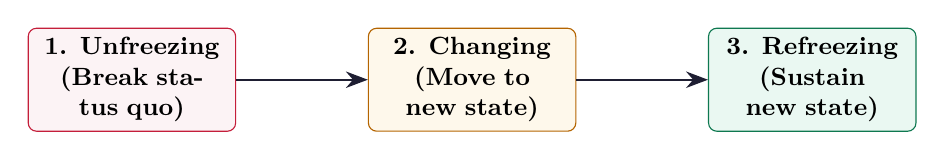
\begin{tikzpicture}[x=1.8cm, y=1.0cm]
  \node [block, fill=hdrred!50, draw=myred] (u) at (0,0) {1. Unfreezing\\(Break status quo)};
  \node [block, fill=hdramber!50, draw=myamber] (c) at (2.4,0) {2. Changing\\(Move to new state)};
  \node [block, fill=hdrgreen!60, draw=mygreen] (r) at (4.8,0) {3. Refreezing\\(Sustain new state)};

  \draw [arrow] (u) -- (c);
  \draw [arrow] (c) -- (r);
\end{tikzpicture}
\end{tcolorbox}

\begin{enumerate}[leftmargin=*, itemsep=3pt]
  \item \textbf{Unfreezing:} Disrupting the existing equilibrium by demonstrating the urgency of change and weakening driving forces of resistance.
  \item \textbf{Changing (Moving):} Implementing new processes, technology, structures, or behaviors.
  \item \textbf{Refreezing:} Institutionalizing the new state by reinforcing positive behaviors through rewards, culture, and policies.
\end{enumerate}

\subsection{Kotter's 8-Step Leading Change Model}
John Kotter proposed an 8-stage strategic framework for executing successful organizational transformations:
\begin{enumerate}[leftmargin=*, itemsep=3pt]
  \item \textbf{Establish Urgency:} Highlight market realities and financial threats to motivate change.
  \item \textbf{Form a Guiding Coalition:} Assemble a powerful team with position power and expertise to lead change.
  \item \textbf{Create a Strategic Vision:} Develop a clear vision and strategic initiatives to direct transformation.
  \item \textbf{Communicate the Vision:} Use all internal channels to communicate the vision and strategy.
  \item \textbf{Empower Broad-Based Action:} Remove structural barriers and revise systems that undermine change.
  \item \textbf{Generate Short-Term Wins:} Plan for visible, unambiguous performance improvements.
  \item \textbf{Sustain Acceleration:} Consolidate gains and produce more change.
  \item \textbf{Institute Change:} Anchor new behaviors in corporate culture and succession planning.
\end{enumerate}

\subsection{Strategies for Overcoming Resistance}
\begin{itemize}[leftmargin=*, itemsep=3pt]
  \item \textbf{Education \& Communication:} Informing employees about change logic to reduce misinformation.
  \item \textbf{Participation \& Involvement:} Involving employees in decision-making to build ownership.
  \item \textbf{Facilitation \& Support:} Providing retraining, counseling, and stress management.
  \item \textbf{Negotiation \& Agreement:} Offering incentives to powerful resistant groups.
\end{itemize}

% ===============================================================================
% 3. ORGANIZATIONAL DEVELOPMENT (OD)
% ===============================================================================
\section{Organizational Development (OD): Concept, Process, and Interventions}

\begin{tcolorbox}[defbox, title={Definition of Organizational Development (OD)}]
  \textbf{Organizational Development (OD)} is a systematic, long-term, top-management-supported effort to improve an organization's vision, empowerment, learning, and problem-solving processes through organizational culture management (Wendell French).
\end{tcolorbox}

\subsection{Core Objectives of OD}
\begin{itemize}[leftmargin=*, itemsep=3pt]
  \item Build high organizational trust, openness, and collaborative problem-solving capacity.
  \item Align organizational structure and culture with technological and strategic demands.
  \item Enhance employee satisfaction, motivation, and personal growth.
\end{itemize}

\subsection{The 4-Stage OD Process}

\begin{tcolorbox}[tikzbox, title={The 4-Stage OD Process}]
\centering
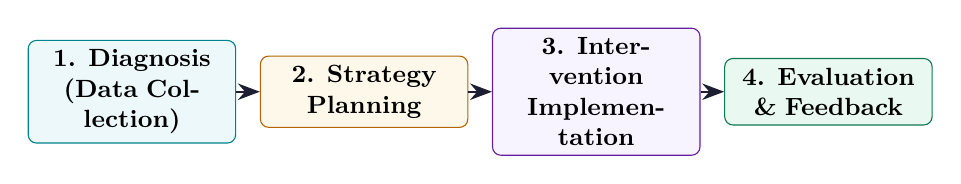
\begin{tikzpicture}[node distance=0.35cm, auto]
  \node [block, fill=hdrteal!50, draw=myteal] (d) {1. Diagnosis\\(Data Collection)};
  \node [block, right=0.3cm of d, fill=hdramber!50, draw=myamber] (s) {2. Strategy\\Planning};
  \node [block, right=0.3cm of s, fill=hdrpurple!40, draw=mypurple] (i) {3. Intervention\\Implementation};
  \node [block, right=0.3cm of i, fill=hdrgreen!60, draw=mygreen] (e) {4. Evaluation\\\& Feedback};

  \draw [arrow] (d) -- (s);
  \draw [arrow] (s) -- (i);
  \draw [arrow] (i) -- (e);
\end{tikzpicture}
\end{tcolorbox}

\subsection{Major OD Interventions}
\par\vspace{6pt}\noindent
\begingroup
\setlength{\tabcolsep}{5pt}%
\setlength{\extrarowheight}{3pt}%
\renewcommand{\arraystretch}{1.35}%
\begin{tabularx}{\linewidth}{|>{\raggedright\arraybackslash\bfseries}p{3.5cm}|Y|}
\hline
\multicolumn{1}{|c|}{\textbf{Intervention Type}} & \multicolumn{1}{c|}{\textbf{Description \& Operational Focus}} \\
\hline
Team Building & Structured activities designed to improve interpersonal trust, goal clarity, and team cohesion. \\
\hline
Sensitivity Training (T-Groups) & Unstructured group interaction sessions aimed at increasing self-awareness and interpersonal sensitivity. \\
\hline
Process Consultation & An outside consultant assists managers in perceiving, understanding, and acting upon process events (e.g., meeting dynamics). \\
\hline
Survey Feedback & Systematic collection of data via questionnaires, followed by feedback sessions to diagnose operational issues. \\
\hline
\end{tabularx}
\endgroup

% ===============================================================================
% QUICK REVISION PAGE
% ===============================================================================
\newpage
\begin{center}
  {\large\bfseries\color{myred} Quick Revision --- Module 4}\\[3pt]
  {\small\color{mydark} Organizational Change \& Development $|$ OE-EC804C}
\end{center}
\vspace{-4pt}
\hrule
\vspace{8pt}

\begin{tcolorbox}[formulabox, title={\textbf{Key Concepts and Metrics at a Glance}}]
\renewcommand{\arraystretch}{1.35}
\begin{tabularx}{\linewidth}{>{\raggedright\arraybackslash\bfseries}p{4.5cm} X}
Lewin's Change Model & 3-stage process: Unfreezing (break status quo) $\to$ Changing (movement) $\to$ Refreezing (institutionalization). \\[4pt]
Resistance Factors & Individual (fear, habit, economic security) vs. Organizational (structural inertia, threat to power). \\[4pt]
OD Definition & Planned, long-term, culture-focused effort to improve organizational effectiveness. \\[4pt]
OD Process Stages & Diagnosis $\to$ Strategy Planning $\to$ Intervention $\to$ Evaluation. \\[4pt]
OD Interventions & Team Building, Sensitivity Training (T-Groups), Process Consultation, Survey Feedback. \\
\end{tabularx}
\end{tcolorbox}

\begin{tcolorbox}[defbox, title={\textbf{One-Line Definitions for Exam Revision}}]
  \begin{itemize}[leftmargin=*, itemsep=2pt]
    \item \textbf{Unfreezing:} Breaking down the existing status quo to prepare individuals for organizational change.
    \item \textbf{Refreezing:} Reinforcing and institutionalizing new behaviors to make change permanent.
    \item \textbf{Process Consultation:} Intervention where a consultant helps managers observe and act upon internal communication and team dynamics.
    \item \textbf{Structural Inertia:} Built-in organizational mechanisms (rules, structure) that act as barriers to change.
  \end{itemize}
\end{tcolorbox}

\begin{tcolorbox}[exambox, title={\textbf{Frequently Asked / Viva Questions}}]
\begin{enumerate}[leftmargin=*, itemsep=4pt]
  \Q{Define Organizational Change. Distinguish between Reactive and Proactive change.}{Organizational change is the alteration of structures, processes, or culture. Reactive change is triggered by immediate external pressure; Proactive change is planned in advance to capture opportunities.}
  
  \Q{Explain Lewin's 3-Step Model of organizational change.}{The model consists of Unfreezing (breaking the status quo), Changing (moving to the new state), and Refreezing (reinforcing and institutionalizing the change).}
  
  \Q{What are the primary individual causes of resistance to change?}{Fear of the unknown, habit, threat to economic security, anxiety over skill competence, and selective perception.}
  
  \Q{What are the primary organizational causes of resistance to change?}{Structural inertia, limited focus of change, threat to specialized expertise, and threat to established power relationships.}
  
  \Q{List four key strategies for overcoming resistance to change.}{Education and communication, employee participation, managerial facilitation and support, and incentive negotiation.}
  
  \Q{Define Organizational Development (OD). What are its main objectives?}{OD is a planned, long-term, top-management-driven effort to improve organizational effectiveness through culture management. Objectives: build trust, openness, and problem-solving capacity.}
  
  \Q{What are the 4 stages of the OD process?}{Diagnosis (data gathering) $\to$ Strategy Planning $\to$ Intervention Execution $\to$ Evaluation and Feedback.}
  
  \Q{Explain Sensitivity Training (T-Groups) as an OD intervention.}{An unstructured group interaction technique designed to increase self-awareness, empathy, and interpersonal communication skills.}
  
  \Q{What is Survey Feedback in OD?}{A diagnostic intervention where data is collected from employees via questionnaires, analyzed, and presented back to teams to identify operational problems.}
  
  \Q{Why is Team Building considered a critical OD intervention?}{It improves interpersonal trust, role clarity, and communication, transforming individual workers into a cohesive, high-performing team.}
\end{enumerate}
\end{tcolorbox}

\end{document}
